\documentclass[aspectratio=169]{beamer}

\usetheme{default}
\usecolortheme{dove}

\setbeamertemplate{navigation symbols}{}
\setbeamertemplate{footline}{%
  \hfill{\large\insertframenumber\,/\,\inserttotalframenumber}\hspace{0.8em}\vspace{0.5em}%
}

\definecolor{popblue}{RGB}{52, 101, 164}
\definecolor{sampred}{RGB}{204, 0, 0}
\definecolor{paramgreen}{RGB}{0, 140, 70}
\definecolor{warnred}{RGB}{180, 40, 40}
\definecolor{orange1}{RGB}{220, 120, 0}
\definecolor{violet1}{RGB}{120, 50, 160}
\definecolor{lightbg}{RGB}{245, 245, 250}

\setbeamercolor{frametitle}{fg=popblue}
\setbeamercolor{title}{fg=popblue}

\usepackage{pgfplots}
\usepackage{tikz}
\usetikzlibrary{shapes, arrows.meta, positioning, calc, decorations.pathreplacing, patterns}
\pgfplotsset{compat=1.18}
\usepackage{amsmath, amssymb}
\usepackage{fontenc}

\title{Lecture 3: Properties of Estimators}
\subtitle{Bias $\cdot$ Variance $\cdot$ MSE $\cdot$ Consistency $\cdot$ Sufficiency $\cdot$ Cram\'er--Rao}
\date{}

\begin{document}

% ============================================================
\begin{frame}
\titlepage
\end{frame}

% ============================================================
\begin{frame}
\frametitle{We use estimators every day. Are they any good?}
\begin{center}
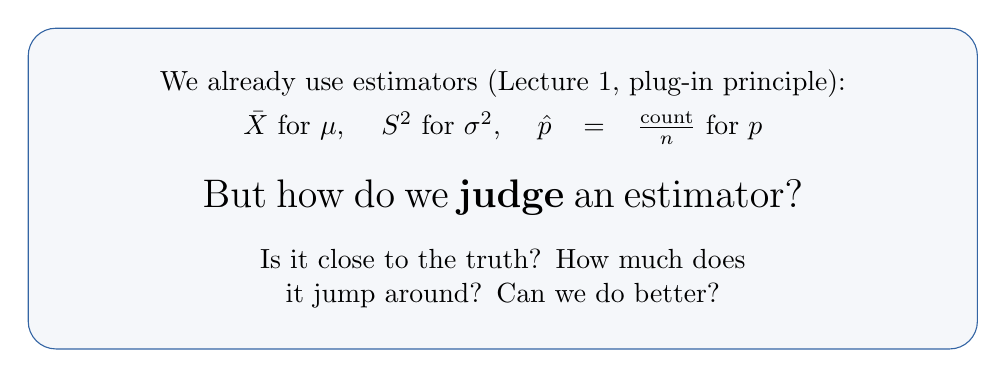
\begin{tikzpicture}
  \node[draw=popblue, fill=popblue!5, rounded corners=10pt, text width=11cm, align=center, inner sep=15pt] {
    We already use estimators (Lecture~1, plug-in principle):\\[4pt]
    $\bar{X}$ for $\mu$, \quad $S^2$ for $\sigma^2$, \quad $\hat{p} = \frac{\text{count}}{n}$ for $p$\\[12pt]
    {\Large But how do we \textbf{judge} an estimator?}\\[10pt]
    Is it close to the truth? How much does it jump around? Can we do better?
  };
\end{tikzpicture}
\end{center}
\end{frame}

% ============================================================
\section{Bias}

\begin{frame}
\frametitle{Bias: Is the Estimator Centered on the Truth?}

$$\text{Bias}(\hat\theta) \;=\; \mathbb{E}[\hat\theta] - \theta$$

\vspace{0.2cm}
\begin{center}
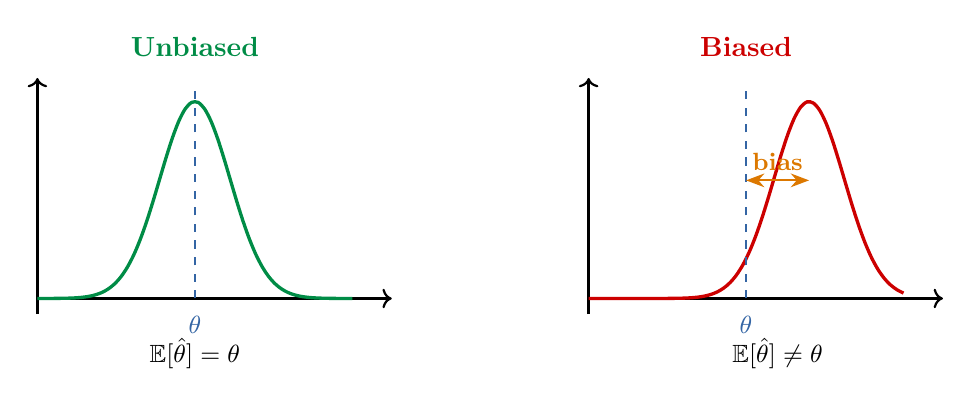
\begin{tikzpicture}
  % Unbiased
  \begin{scope}[xshift=-5cm]
    \node[font=\bfseries, paramgreen] at (2, 3.2) {Unbiased};
    \draw[thick, ->] (0, 0) -- (4.5, 0);
    \draw[thick, ->] (0, -0.2) -- (0, 2.8);
    \draw[very thick, paramgreen, smooth, domain=0:4, samples=50] plot (\x, {2.5*exp(-(\x-2)*(\x-2)/0.4)});
    \draw[dashed, thick, popblue] (2, 0) -- (2, 2.7);
    \node[below, font=\small, popblue] at (2, -0.1) {$\theta$};
    \node[font=\small] at (2, -0.7) {$\mathbb{E}[\hat\theta] = \theta$};
  \end{scope}

  % Biased
  \begin{scope}[xshift=2cm]
    \node[font=\bfseries, sampred] at (2, 3.2) {Biased};
    \draw[thick, ->] (0, 0) -- (4.5, 0);
    \draw[thick, ->] (0, -0.2) -- (0, 2.8);
    \draw[very thick, sampred, smooth, domain=0:4, samples=50] plot (\x, {2.5*exp(-(\x-2.8)*(\x-2.8)/0.4)});
    \draw[dashed, thick, popblue] (2, 0) -- (2, 2.7);
    \node[below, font=\small, popblue] at (2, -0.1) {$\theta$};
    \draw[{Stealth}-{Stealth}, thick, orange1] (2, 1.5) -- (2.8, 1.5);
    \node[above, font=\small\bfseries, orange1] at (2.4, 1.5) {bias};
    \node[font=\small] at (2.4, -0.7) {$\mathbb{E}[\hat\theta] \neq \theta$};
  \end{scope}
\end{tikzpicture}
\end{center}

\vspace{0.1cm}
\begin{center}
\small If $\text{Bias}(\hat\theta) = 0$ for all $\theta$, the estimator is \textbf{unbiased}.
\end{center}
\end{frame}

\begin{frame}
\frametitle{Worked Example: Is $\bar{X}$ Unbiased for $\mu$?}

Let $X_1, \ldots, X_n$ be i.i.d.\ with $\mathbb{E}[X_i] = \mu$. \;Is $\hat\mu = \bar{X} = \frac{1}{n}\sum_{i=1}^n X_i$ unbiased?

\vspace{0.3cm}
\textbf{Step 1:} Compute $\mathbb{E}[\hat\mu]$:
$$\mathbb{E}[\bar{X}] = \mathbb{E}\!\left[\frac{1}{n}\sum_{i=1}^n X_i\right]
= \frac{1}{n}\sum_{i=1}^n \mathbb{E}[X_i]
= \frac{1}{n}\cdot n\mu = \mu$$

\pause
\textbf{Step 2:} Check bias:
$$\text{Bias}(\bar{X}) = \mathbb{E}[\bar{X}] - \mu = \mu - \mu = 0 \quad\textcolor{paramgreen}{\checkmark\;\text{Unbiased!}}$$

\vspace{0.2cm}
\begin{center}
\fcolorbox{popblue}{popblue!5}{\parbox{11cm}{\centering\small
  \textbf{Recipe for any estimator:}\\
  (1)~Compute $\mathbb{E}[\hat\theta]$ \;\;$\to$\;\; (2)~Subtract the true $\theta$ \;\;$\to$\;\; (3)~If the result is $0$, it's unbiased.
}}
\end{center}
\end{frame}

% --- Item 1: More detailed bias derivation ---
\begin{frame}
\frametitle{Worked Example: Why Dividing by $n$ Is Biased}

\small
We want to estimate $\sigma^2 = \text{Var}(X_i)$. Natural guess: $\hat\sigma^2_n = \frac{1}{n}\sum_{i=1}^n (X_i - \bar{X})^2$.

\vspace{0.1cm}
\textbf{Trick:} rewrite each $(X_i - \bar{X})$ by adding and subtracting the true mean $\mu$:
$$X_i - \bar{X} = \underbrace{(X_i - \mu)}_{\text{deviation from truth}} - \underbrace{(\bar{X} - \mu)}_{\text{estimation error}}$$

Squaring and summing gives the \textbf{key identity}:
$$\sum_{i=1}^n (X_i - \bar{X})^2 = \sum_{i=1}^n(X_i - \mu)^2 \;-\; n(\bar{X} - \mu)^2$$

\pause
\vspace{-0.1cm}
\textbf{Take expectations} (using $\mathbb{E}[(X_i - \mu)^2] = \sigma^2$ and $\text{Var}(\bar{X}) = \sigma^2/n$):

\vspace{-0.3cm}
\begin{align*}
  \mathbb{E}\!\left[\textstyle\sum(X_i - \mu)^2\right] &= n\sigma^2 &\text{($n$ terms, each $\sigma^2$)}\\[-3pt]
  \mathbb{E}\!\left[n(\bar{X} - \mu)^2\right] &= n \cdot \text{Var}(\bar{X}) = n \cdot \frac{\sigma^2}{n} = \textcolor{orange1}{\sigma^2} &\text{(one ``lost'' degree of freedom)}
\end{align*}

\vspace{-0.4cm}
$$\Rightarrow\quad\mathbb{E}\!\left[\textstyle\sum(X_i - \bar{X})^2\right] = n\sigma^2 - \textcolor{orange1}{\sigma^2} = \textcolor{sampred}{(n-1)\sigma^2}$$
\end{frame}

\begin{frame}
\frametitle{Bessel's Correction: The Fix}

\small
From the previous slide: $\mathbb{E}\!\left[\sum(X_i - \bar{X})^2\right] = (n{-}1)\sigma^2$, so:

\vspace{0.2cm}
\begin{center}
\fcolorbox{sampred}{sampred!5}{\parbox{11cm}{\centering
  $\mathbb{E}[\hat\sigma^2_n] = \mathbb{E}\!\left[\frac{1}{n}\sum(X_i - \bar{X})^2\right] = \frac{(n-1)\sigma^2}{n} \neq \sigma^2$ \quad\textcolor{sampred}{\textbf{Biased!}}\\[4pt]
  \small It \textbf{underestimates} by $\sigma^2/n$. \;Why? We used $\bar{X}$ instead of $\mu$, ``using up'' one degree of freedom.
}}
\end{center}

\vspace{0.3cm}
\begin{center}
\fcolorbox{paramgreen}{paramgreen!5}{\parbox{11cm}{\centering
  \textbf{Bessel's correction:} Divide by $n{-}1$ instead of $n$:\\[4pt]
  $S^2 = \frac{1}{n-1}\sum_{i=1}^n(X_i - \bar{X})^2$ \qquad $\mathbb{E}[S^2] = \sigma^2$ \;\;\textcolor{paramgreen}{$\checkmark$ Unbiased!}
}}
\end{center}

\vspace{0.2cm}
\begin{center}
\small\textbf{Intuition:} We estimated $\mu$ from the same data, so the residuals $(X_i - \bar{X})$\\
are ``too small'' on average. Dividing by $n{-}1$ corrects for this.
\end{center}
\end{frame}

\begin{frame}
\frametitle{Bias: Summary}

\renewcommand{\arraystretch}{1.8}
\begin{center}
\begin{tabular}{lcc}
  \textbf{Estimator} & \textbf{Bias} & \textbf{Unbiased?} \\
  \hline
  $\bar{X} = \frac{1}{n}\sum X_i$ \;\text{for}\; $\mu$ &
  $0$ &
  \textcolor{paramgreen}{\textbf{Yes}} \\
  $\hat\sigma^2_n = \frac{1}{n}\sum(X_i-\bar{X})^2$ \;\text{for}\; $\sigma^2$ &
  $-\frac{\sigma^2}{n}$ &
  \textcolor{sampred}{\textbf{No}} \\
  $S^2 = \frac{1}{n-1}\sum(X_i-\bar{X})^2$ \;\text{for}\; $\sigma^2$ &
  $0$ &
  \textcolor{paramgreen}{\textbf{Yes}} \\
  $\hat{p} = \frac{\sum X_i}{n}$ \;\text{for}\; $p$ (Bernoulli) &
  $0$ &
  \textcolor{paramgreen}{\textbf{Yes}} \\
  \hline
\end{tabular}
\end{center}

\vspace{0.3cm}
\begin{center}
\fcolorbox{orange1}{orange1!5}{\parbox{10cm}{\centering\small
  Dividing by $n$ instead of $n{-}1$ \textbf{underestimates} the true variance.\\
  Bessel's correction ($n{-}1$) fixes this. Recall Lecture~2!
}}
\end{center}
\end{frame}

\begin{frame}
\frametitle{Unbiasedness Alone Isn't Enough}

Consider estimating $\mu = \mathbb{E}[X_i]$ from $X_1, \ldots, X_n$.

\vspace{0.2cm}
\textbf{Surprising fact:} $\tilde\mu = X_1$ is also \textbf{unbiased}!
$$\mathbb{E}[X_1] = \mu \quad\Rightarrow\quad \text{Bias}(X_1) = 0 \quad\textcolor{paramgreen}{\checkmark}$$

\pause
But it's a terrible estimator --- it ignores $X_2, \ldots, X_n$ entirely!

\vspace{0.2cm}
\begin{center}
\fcolorbox{orange1}{orange1!5}{\parbox{11cm}{\centering\small
  \textbf{Three statisticians go deer hunting.}\\[3pt]
  The first one shoots \textbf{1 meter to the left} of the deer.\\
  The second one shoots \textbf{1 meter to the right}.\\
  The third one shouts: \textit{``We got it!''}\\[4pt]
  On average they hit the target --- \textbf{unbiased!} But not very useful\ldots
}}
\end{center}

\vspace{0.15cm}
\begin{center}
\small\textbf{Lesson:} Unbiasedness only says $\mathbb{E}[\hat\theta] = \theta$. It says nothing about\\
how much $\hat\theta$ \textbf{varies}. We need more: \textbf{variance} and \textbf{MSE}.
\end{center}
\end{frame}

% ============================================================
\section{Variance and MSE}

\begin{frame}
\frametitle{The Dartboard Analogy}
\vspace{-0.2cm}
\begin{center}
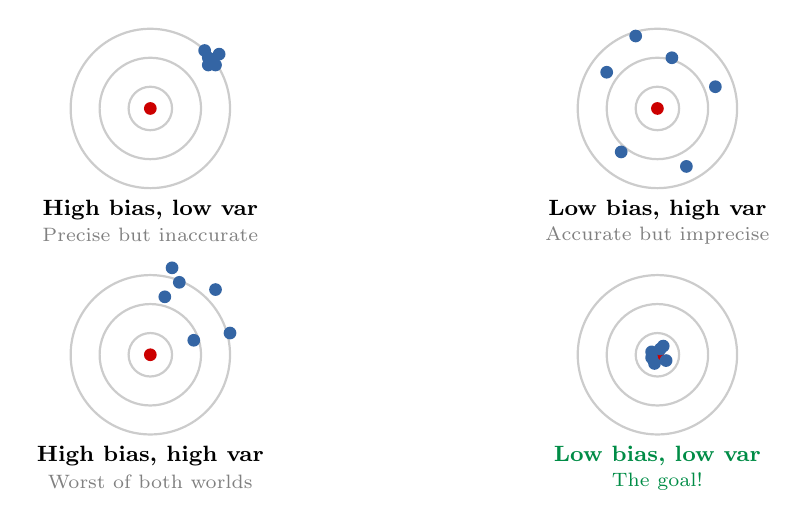
\begin{tikzpicture}[scale=0.92]
  % --- Top-left: High bias, low variance ---
  \begin{scope}[xshift=-3.5cm, yshift=1.2cm]
    \draw[thick, gray!40] (0,0) circle (1.1);
    \draw[thick, gray!40] (0,0) circle (0.7);
    \draw[thick, gray!40] (0,0) circle (0.3);
    \fill[sampred] (0,0) circle (2.5pt);
    \foreach \x/\y in {0.8/0.7, 0.9/0.6, 0.75/0.8, 0.85/0.65, 0.95/0.75, 0.8/0.6} {
      \fill[popblue] (\x, \y) circle (2.5pt);
    }
    \node[font=\footnotesize\bfseries] at (0, -1.4) {High bias, low var};
    \node[font=\scriptsize, gray] at (0, -1.75) {Precise but inaccurate};
  \end{scope}

  % --- Top-right: Low bias, high variance ---
  \begin{scope}[xshift=3.5cm, yshift=1.2cm]
    \draw[thick, gray!40] (0,0) circle (1.1);
    \draw[thick, gray!40] (0,0) circle (0.7);
    \draw[thick, gray!40] (0,0) circle (0.3);
    \fill[sampred] (0,0) circle (2.5pt);
    \foreach \x/\y in {-0.7/0.5, 0.4/-0.8, -0.3/1.0, 0.8/0.3, -0.5/-0.6, 0.2/0.7} {
      \fill[popblue] (\x, \y) circle (2.5pt);
    }
    \node[font=\footnotesize\bfseries] at (0, -1.4) {Low bias, high var};
    \node[font=\scriptsize, gray] at (0, -1.75) {Accurate but imprecise};
  \end{scope}

  % --- Bottom-left: High bias, high variance ---
  \begin{scope}[xshift=-3.5cm, yshift=-2.2cm]
    \draw[thick, gray!40] (0,0) circle (1.1);
    \draw[thick, gray!40] (0,0) circle (0.7);
    \draw[thick, gray!40] (0,0) circle (0.3);
    \fill[sampred] (0,0) circle (2.5pt);
    \foreach \x/\y in {0.4/1.0, 1.1/0.3, 0.2/0.8, 0.9/0.9, 0.6/0.2, 0.3/1.2} {
      \fill[popblue] (\x, \y) circle (2.5pt);
    }
    \node[font=\footnotesize\bfseries] at (0, -1.4) {High bias, high var};
    \node[font=\scriptsize, gray] at (0, -1.75) {Worst of both worlds};
  \end{scope}

  % --- Bottom-right: Low bias, low variance ---
  \begin{scope}[xshift=3.5cm, yshift=-2.2cm]
    \draw[thick, gray!40] (0,0) circle (1.1);
    \draw[thick, gray!40] (0,0) circle (0.7);
    \draw[thick, gray!40] (0,0) circle (0.3);
    \fill[sampred] (0,0) circle (2.5pt);
    \foreach \x/\y in {0.08/0.12, -0.08/-0.04, 0.04/0.08, -0.04/-0.12, 0.12/-0.08, -0.08/0.04} {
      \fill[popblue] (\x, \y) circle (2.5pt);
    }
    \node[font=\footnotesize\bfseries, paramgreen] at (0, -1.4) {Low bias, low var};
    \node[font=\scriptsize, paramgreen] at (0, -1.75) {The goal!};
  \end{scope}
\end{tikzpicture}
\end{center}
\vspace{-0.2cm}
\begin{center}
\small \textcolor{sampred}{Bullseye} = true $\theta$. \;\textcolor{popblue}{Blue dots} = estimates from repeated samples.
\end{center}
\end{frame}

% --- Item 2: Explain why sigma^2/n ---
\begin{frame}
\frametitle{Variance of an Estimator}

The \textbf{variance} measures how much $\hat\theta$ wobbles across samples:
$\text{Var}(\hat\theta) = \mathbb{E}\!\left[(\hat\theta - \mathbb{E}[\hat\theta])^2\right]$

\vspace{0.05cm}
\textbf{Why is $\text{Var}(\bar{X}) = \sigma^2/n$ and not $\sigma^2/n^2$?}

\vspace{-0.2cm}
\begin{align*}
  \text{Var}(\bar{X})
  &= \text{Var}\!\left(\frac{1}{n}\sum_{i=1}^n X_i\right)
  = \frac{1}{n^2}\,\text{Var}\!\left(\sum_{i=1}^n X_i\right) &\text{($\frac{1}{n}$ comes out as $\frac{1}{n^2}$)}\\[2pt]
  &= \frac{1}{n^2}\sum_{i=1}^n \text{Var}(X_i) &\text{(independent $\Rightarrow$ variances \textbf{add})}\\[2pt]
  &= \frac{1}{n^2}\cdot n\sigma^2 = \boxed{\frac{\sigma^2}{n}} &\text{($n$ terms cancel one $n$)}
\end{align*}

\vspace{-0.3cm}
\begin{center}
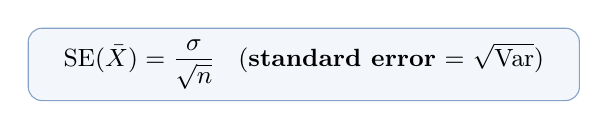
\begin{tikzpicture}[
  ebox/.style={draw=popblue!60, fill=popblue!6, rounded corners=5pt, minimum width=7cm, align=center, font=\small, inner sep=4pt}
]
  \node[ebox] at (0, 0) {$\text{SE}(\bar{X}) = \dfrac{\sigma}{\sqrt{n}}$ \;\;(\textbf{standard error} = $\sqrt{\text{Var}}$)};
\end{tikzpicture}
\end{center}
\end{frame}

% --- Item 3: MSE split into 2 slides ---
\begin{frame}
\frametitle{Mean Squared Error: The Total Error}

\small
Bias tells us about the \textbf{aim}, variance about the \textbf{spread}. Can we combine them?

\vspace{0.2cm}
\begin{center}
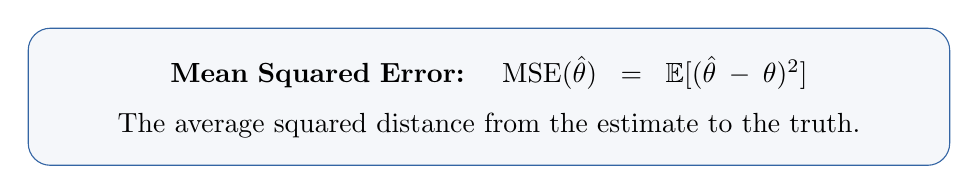
\begin{tikzpicture}
  \node[draw=popblue, fill=popblue!5, rounded corners=8pt, text width=11cm, align=center, inner sep=10pt] {
    \textbf{Mean Squared Error:} $\;\text{MSE}(\hat\theta) = \mathbb{E}[(\hat\theta - \theta)^2]$\\[6pt]
    The average squared distance from the estimate to the truth.
  };
\end{tikzpicture}
\end{center}

\vspace{0.2cm}
\textbf{The trick:} add and subtract $\mathbb{E}[\hat\theta]$ to decompose the error:
$$\hat\theta - \theta
  = \underbrace{(\hat\theta - \mathbb{E}[\hat\theta])}_{\text{random fluctuation}} + \underbrace{(\mathbb{E}[\hat\theta] - \theta)}_{\text{bias (a constant!)}}$$

\vspace{0.2cm}
\begin{center}
\fcolorbox{orange1}{orange1!5}{\parbox{11cm}{\centering\small
  This splits the total error into two pieces: the \textbf{random part} (how much $\hat\theta$ moves around its own mean)
  and the \textbf{systematic part} (how far that mean is from the truth).
}}
\end{center}
\end{frame}

\begin{frame}
\frametitle{MSE = Bias$^2$ + Variance: The Proof}

\small
Now square $\hat\theta - \theta = (\hat\theta - \mathbb{E}[\hat\theta]) + (\mathbb{E}[\hat\theta] - \theta)$ and take expectations:

\vspace{-0.1cm}
\begin{align*}
  \mathbb{E}[(\hat\theta - \theta)^2]
  &= \mathbb{E}\!\left[(\hat\theta - \mathbb{E}[\hat\theta])^2\right]
   + 2\underbrace{(\mathbb{E}[\hat\theta] - \theta)}_{\text{constant}} \cdot\underbrace{\mathbb{E}[\hat\theta - \mathbb{E}[\hat\theta]]}_{= \,0\text{ (always!)}}
   + (\mathbb{E}[\hat\theta] - \theta)^2
\end{align*}

\vspace{-0.3cm}
The cross term vanishes because $\hat\theta - \mathbb{E}[\hat\theta]$ has mean zero \textbf{by definition}.

\vspace{0.1cm}
$$\boxed{\text{MSE}(\hat\theta) = \text{Var}(\hat\theta) + \text{Bias}^2(\hat\theta)}$$

\vspace{0.1cm}
\begin{center}
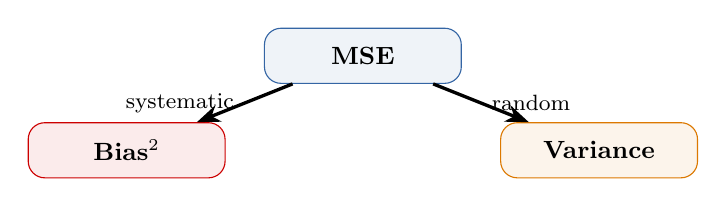
\begin{tikzpicture}
  \node[draw=popblue, fill=popblue!8, rounded corners=6pt, minimum width=2.5cm, minimum height=0.7cm, font=\small] (mse) at (0, 0) {\textbf{MSE}};
  \node[draw=sampred, fill=sampred!8, rounded corners=6pt, minimum width=2.5cm, minimum height=0.7cm, font=\small] (bias) at (-3, -1.2) {\textbf{Bias}$^2$};
  \node[draw=orange1, fill=orange1!8, rounded corners=6pt, minimum width=2.5cm, minimum height=0.7cm, font=\small] (var) at (3, -1.2) {\textbf{Variance}};
  \draw[-{Stealth}, very thick] (mse) -- (bias) node[midway, left, font=\footnotesize] {systematic};
  \draw[-{Stealth}, very thick] (mse) -- (var) node[midway, right, font=\footnotesize] {random};
\end{tikzpicture}
\end{center}

\vspace{-0.05cm}
\begin{center}
\small Unbiased means $\text{MSE} = \text{Var}$, but a biased estimator can still win if its variance is low enough.
\end{center}
\end{frame}

\begin{frame}
\frametitle{When Biased Beats Unbiased}

\textbf{Example:} Estimating $\sigma^2$ from $X_1,\ldots,X_n \sim N(\mu, \sigma^2)$.

\vspace{0.2cm}
\begin{center}
\renewcommand{\arraystretch}{1.6}
\begin{tabular}{lccc}
  \textbf{Estimator} & \textbf{Bias} & \textbf{Variance} & \textbf{MSE} \\
  \hline
  $S^2 = \frac{1}{n-1}\sum(X_i - \bar{X})^2$ & $0$ & $\frac{2\sigma^4}{n-1}$ & $\frac{2\sigma^4}{n-1}$ \\[6pt]
  $\hat\sigma^2_n = \frac{1}{n}\sum(X_i - \bar{X})^2$ & $-\frac{\sigma^2}{n}$ & $\frac{2(n-1)\sigma^4}{n^2}$ & $\frac{(2n-1)\sigma^4}{n^2}$ \\[6pt]
  \hline
\end{tabular}
\end{center}

\vspace{0.2cm}
\begin{center}
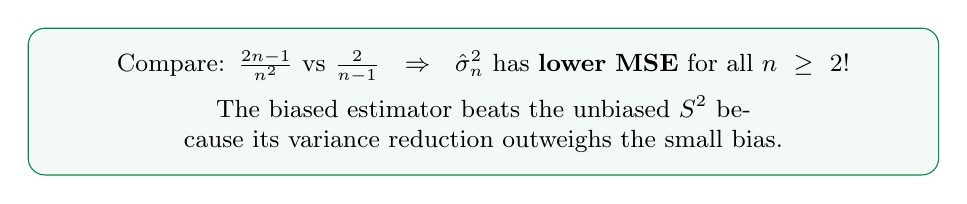
\begin{tikzpicture}
  \node[draw=paramgreen, fill=paramgreen!5, rounded corners=6pt, text width=11cm, align=center, inner sep=8pt, font=\small] {
    Compare: $\frac{2n-1}{n^2}$ vs $\frac{2}{n-1}$ $\;\Rightarrow\;$ $\hat\sigma^2_n$ has \textbf{lower MSE} for all $n \geq 2$!\\[4pt]
    The biased estimator beats the unbiased $S^2$ because its variance reduction outweighs the small bias.
  };
\end{tikzpicture}
\end{center}
\end{frame}

% Item 4: MSE Comparison Visualized slide REMOVED

% ============================================================
% --- Item 5 + Item 6: Bias-Variance Tradeoff (2 slides, Armenian colors, ML connection) ---
\section{Bias-Variance Tradeoff}

\begin{frame}
\begin{center}
\vspace{1cm}
{\LARGE\bfseries\textcolor{popblue}{The Bias-Variance Tradeoff}}\\[15pt]
{\large You can't minimize bias and variance at the same time.}\\[8pt]
{\large How do we find the \textbf{sweet spot}?}
\end{center}
\end{frame}

\begin{frame}
\frametitle{The Bias-Variance Tradeoff}
\begin{center}
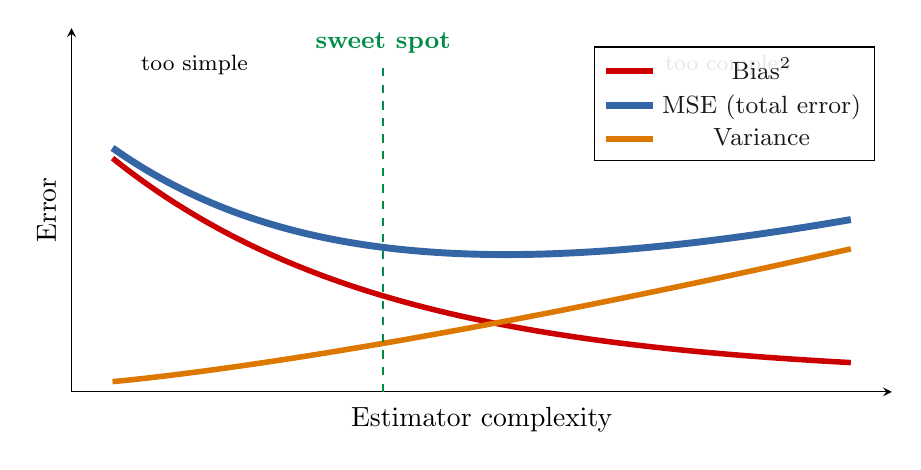
\begin{tikzpicture}
  \begin{axis}[
    width=12cm, height=6.2cm,
    xlabel={Estimator complexity},
    ylabel={Error},
    xmin=0, xmax=10,
    ymin=0, ymax=5,
    xtick=\empty,
    ytick=\empty,
    axis lines=left,
    every axis plot/.append style={line width=2pt, smooth, samples=50},
    legend style={at={(0.98,0.95)}, anchor=north east, font=\small, fill=white, fill opacity=0.9},
  ]
    % Armenian flag order: red, blue, orange
    % Bias^2 (decreasing) - RED
    \addplot[sampred, domain=0.5:9.5] {3.5*exp(-0.3*x) + 0.2};
    \addlegendentry{Bias$^2$}

    % MSE (U-shaped) - BLUE
    \addplot[popblue, domain=0.5:9.5, line width=2.5pt] {3.5*exp(-0.3*x) + 0.1*x^1.3 + 0.3};
    \addlegendentry{MSE (total error)}

    % Variance (increasing) - ORANGE
    \addplot[orange1, domain=0.5:9.5] {0.1*x^1.3 + 0.1};
    \addlegendentry{Variance}

    % Optimal point
    \draw[dashed, thick, paramgreen] (axis cs:3.8, 0) -- (axis cs:3.8, 4.5);
    \node[font=\small\bfseries, paramgreen] at (axis cs:3.8, 4.8) {sweet spot};

    % Annotations
    \node[font=\footnotesize] at (axis cs:1.5, 4.5) {too simple};
    \node[font=\footnotesize] at (axis cs:8, 4.5) {too complex};
  \end{axis}
\end{tikzpicture}
\end{center}
\end{frame}

\begin{frame}
\frametitle{Bias-Variance in Machine Learning}

\small
This tradeoff is \textbf{everywhere} in ML --- it's the same principle in different disguises:

\vspace{0.1cm}
\begin{center}
\renewcommand{\arraystretch}{1.5}
\begin{tabular}{lll}
  \textbf{Setting} & \textbf{Too simple (high bias)} & \textbf{Too complex (high var)} \\
  \hline
  Polynomial regression & Degree 1 (line) & Degree 20 (wiggly) \\
  KNN & Large $k$ (oversmoothed) & $k=1$ (memorizes noise) \\
  Decision tree & Shallow tree (underfits) & Deep tree (overfits) \\
  Neural network & Too few neurons & Too many neurons \\
  Regularization & Strong penalty ($\lambda$ large) & No penalty ($\lambda = 0$) \\
  \hline
\end{tabular}
\end{center}

\vspace{0.1cm}
\begin{center}
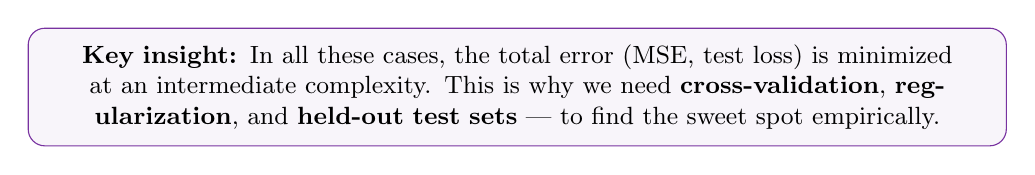
\begin{tikzpicture}
  \node[draw=violet1, fill=violet1!5, rounded corners=6pt, text width=12cm, align=center, inner sep=6pt, font=\small] {
    \textbf{Key insight:} In all these cases, the total error (MSE, test loss) is minimized at an
    intermediate complexity. This is why we need \textbf{cross-validation}, \textbf{regularization},
    and \textbf{held-out test sets} --- to find the sweet spot empirically.
  };
\end{tikzpicture}
\end{center}
\end{frame}

% ============================================================
% --- Items 6, 7, 8: Consistency (transition, expanded, extra slide) ---
\section{Consistency}

\begin{frame}
\begin{center}
\vspace{1cm}
{\LARGE\bfseries\textcolor{popblue}{Consistency}}\\[15pt]
{\large Does our estimator converge to the truth}\\[4pt]
{\large as we collect more and more data?}
\end{center}
\end{frame}

\begin{frame}
\frametitle{Consistency: Getting It Right Eventually}

An estimator $\hat\theta_n$ is \textbf{consistent} if it converges to the truth as $n \to \infty$:
$$\hat\theta_n \xrightarrow{P} \theta \qquad\text{i.e.,}\quad \Pr\!\left(|\hat\theta_n - \theta| > \varepsilon\right) \to 0 \;\;\text{for all } \varepsilon > 0$$

\vspace{0.3cm}
\begin{center}
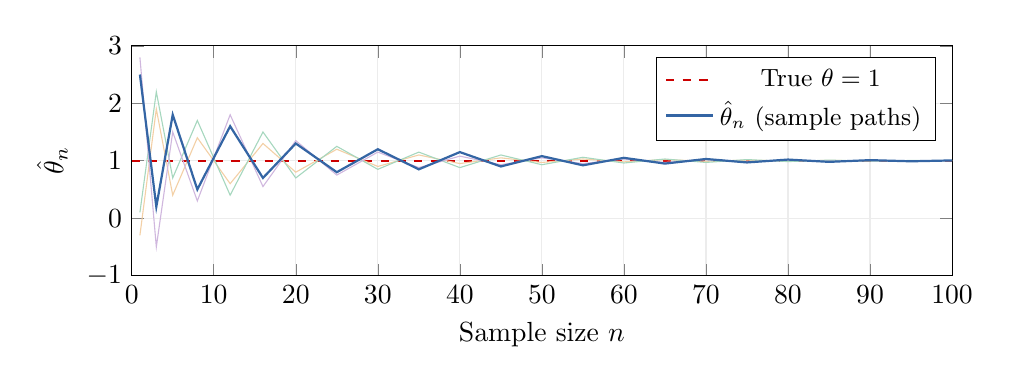
\begin{tikzpicture}
  \begin{axis}[
    width=12cm, height=4.5cm,
    xlabel={Sample size $n$},
    ylabel={$\hat\theta_n$},
    xmin=0, xmax=100,
    ymin=-1, ymax=3,
    grid=major, grid style={gray!15},
    legend style={at={(0.98,0.95)}, anchor=north east, font=\small},
  ]
    % True value
    \addplot[dashed, thick, sampred, domain=0:100] {1};
    \addlegendentry{True $\theta = 1$}

    % Faded sample paths
    \addplot[orange1!35, thin, mark=none, forget plot] coordinates {
      (1, -0.3) (3, 1.9) (5, 0.4) (8, 1.4) (12, 0.6) (16, 1.3)
      (20, 0.8) (25, 1.2) (30, 0.9) (35, 1.1) (40, 0.95)
      (45, 1.05) (50, 0.97) (55, 1.03) (60, 0.98) (65, 1.02)
      (70, 0.99) (75, 1.01) (80, 0.995) (85, 1.005) (90, 0.998) (95, 1.002) (100, 1.001)
    };
    \addplot[paramgreen!35, thin, mark=none, forget plot] coordinates {
      (1, 0.1) (3, 2.2) (5, 0.7) (8, 1.7) (12, 0.4) (16, 1.5)
      (20, 0.7) (25, 1.25) (30, 0.85) (35, 1.15) (40, 0.88)
      (45, 1.1) (50, 0.93) (55, 1.06) (60, 0.96) (65, 1.03)
      (70, 0.97) (75, 1.02) (80, 0.985) (85, 1.01) (90, 0.993) (95, 1.004) (100, 0.998)
    };
    \addplot[violet1!35, thin, mark=none, forget plot] coordinates {
      (1, 2.8) (3, -0.5) (5, 1.5) (8, 0.3) (12, 1.8) (16, 0.55)
      (20, 1.35) (25, 0.75) (30, 1.15) (35, 0.88) (40, 1.08)
      (45, 0.93) (50, 1.05) (55, 0.95) (60, 1.03) (65, 0.97)
      (70, 1.02) (75, 0.98) (80, 1.01) (85, 0.99) (90, 1.005) (95, 0.997) (100, 1.002)
    };

    % Main sample path
    \addplot[popblue, thick, mark=none] coordinates {
      (1, 2.5) (3, 0.2) (5, 1.8) (8, 0.5) (12, 1.6) (16, 0.7)
      (20, 1.3) (25, 0.8) (30, 1.2) (35, 0.85) (40, 1.15)
      (45, 0.9) (50, 1.08) (55, 0.92) (60, 1.05) (65, 0.95)
      (70, 1.03) (75, 0.97) (80, 1.02) (85, 0.98) (90, 1.01) (95, 0.99) (100, 1.005)
    };
    \addlegendentry{$\hat\theta_n$ (sample paths)}
  \end{axis}
\end{tikzpicture}
\end{center}
\end{frame}

% --- Item 8: Extra consistency slide ---
\begin{frame}
\frametitle{Consistent vs Inconsistent: A Contrast}

\small
\begin{columns}[T]
\begin{column}{0.48\textwidth}
\begin{center}
\textcolor{paramgreen}{\textbf{Consistent:}} $\hat\mu = \bar{X}_n$
\end{center}
\begin{itemize}\setlength{\itemsep}{2pt}
  \item $\mathbb{E}[\bar{X}_n] = \mu$ \;(unbiased)
  \item $\text{Var}(\bar{X}_n) = \sigma^2/n \to 0$
  \item Uses \textbf{all} $n$ observations
  \item More data $\Rightarrow$ more precise
\end{itemize}
\end{column}
\begin{column}{0.48\textwidth}
\begin{center}
\textcolor{sampred}{\textbf{Not consistent:}} $\tilde\mu = X_1$
\end{center}
\begin{itemize}\setlength{\itemsep}{2pt}
  \item $\mathbb{E}[X_1] = \mu$ \;(also unbiased!)
  \item $\text{Var}(X_1) = \sigma^2$ \;(constant!)
  \item Uses \textbf{only} the first observation
  \item Ignores all other data forever
\end{itemize}
\end{column}
\end{columns}

\vspace{0.3cm}
\begin{center}
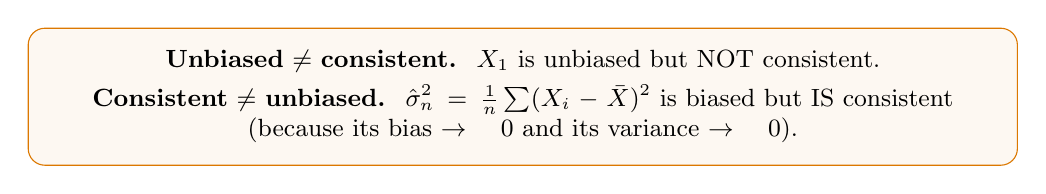
\begin{tikzpicture}
  \node[draw=orange1, fill=orange1!5, rounded corners=6pt, text width=12cm, align=center, inner sep=8pt, font=\small] {
    \textbf{Unbiased $\neq$ consistent.} \;$X_1$ is unbiased but NOT consistent.\\[3pt]
    \textbf{Consistent $\neq$ unbiased.} \;$\hat\sigma^2_n = \frac{1}{n}\sum(X_i - \bar{X})^2$ is biased but IS consistent\\
    (because its bias $\to 0$ and its variance $\to 0$).
  };
\end{tikzpicture}
\end{center}
\end{frame}

% --- Item 7: Chebyshev explanation for consistency ---
\begin{frame}
\frametitle{Sufficient Conditions for Consistency}

\small
\textbf{Chebyshev's inequality} gives us a concrete tool:
\vspace{-0.2cm}
$$\Pr\!\left(|\hat\theta_n - \theta| \geq \varepsilon\right) \;\leq\; \frac{\mathbb{E}[(\hat\theta_n - \theta)^2]}{\varepsilon^2} = \frac{\text{MSE}(\hat\theta_n)}{\varepsilon^2} = \frac{\text{Bias}^2 + \text{Var}}{\varepsilon^2}$$

\vspace{-0.25cm}
\begin{center}
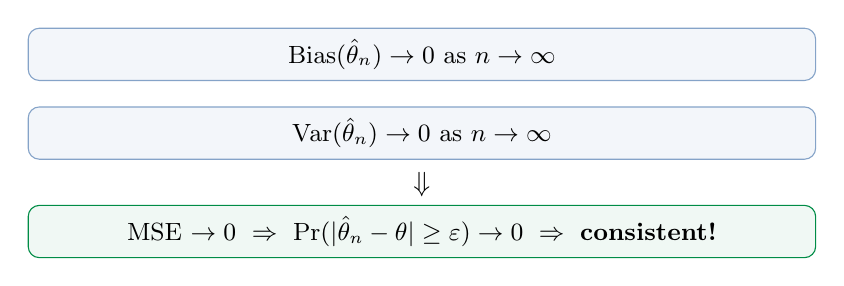
\begin{tikzpicture}[
  sbox/.style={draw=popblue!60, fill=popblue!6, rounded corners=4pt, minimum width=10cm, align=center, font=\small, inner sep=4pt}
]
  \node[sbox] at (0, 1.1) {$\text{Bias}(\hat\theta_n) \to 0$ as $n \to \infty$};
  \node[sbox] at (0, 0.1) {$\text{Var}(\hat\theta_n) \to 0$ as $n \to \infty$};
  \node[font=\normalsize] at (0, -0.55) {$\Downarrow$};
  \node[draw=paramgreen, fill=paramgreen!6, rounded corners=4pt, minimum width=10cm, align=center, font=\small, inner sep=4pt]
    at (0, -1.15) {MSE $\to 0$ \;$\Rightarrow$\; $\Pr(|\hat\theta_n - \theta| \geq \varepsilon) \to 0$ \;$\Rightarrow$\; \textbf{consistent!}};
\end{tikzpicture}
\end{center}

\vspace{-0.1cm}
\small\textbf{Example:} $\bar{X}_n$ is consistent for $\mu$: $\text{Bias} = 0$, $\text{Var} = \sigma^2/n \to 0$, so $\Pr(|\bar{X}_n - \mu| \geq \varepsilon) \leq \sigma^2/(n\varepsilon^2) \to 0$.

\vspace{0.05cm}
\centering\small This is precisely the \textbf{(Weak) Law of Large Numbers}: $\bar{X}_n \xrightarrow{P} \mu$.
\end{frame}

% \begin{frame}
% \frametitle{Worked Example: Is $\hat\sigma^2_n$ Consistent?}

% \small
% We know $\hat\sigma^2_n = \frac{1}{n}\sum(X_i - \bar{X})^2$ is \textbf{biased} for $\sigma^2$. But is it \textbf{consistent}?

% \vspace{0.15cm}
% \textbf{Step 1:} Check bias as $n \to \infty$:
% $$\text{Bias}(\hat\sigma^2_n) = -\frac{\sigma^2}{n} \;\xrightarrow{n\to\infty}\; 0 \quad\textcolor{paramgreen}{\checkmark}$$

% \pause
% \textbf{Step 2:} Check variance as $n \to \infty$ (for Normal data):
% $$\text{Var}(\hat\sigma^2_n) = \frac{2(n-1)\sigma^4}{n^2} \;\xrightarrow{n\to\infty}\; 0 \quad\textcolor{paramgreen}{\checkmark}$$

% \pause
% \textbf{Step 3:} Apply the sufficient condition:
% $$\text{MSE}(\hat\sigma^2_n) = \underbrace{\text{Bias}^2}_{\to\,0} + \underbrace{\text{Var}}_{\to\,0} \;\to\; 0$$

% \vspace{0.1cm}
% \begin{center}
% \fcolorbox{paramgreen}{paramgreen!5}{\parbox{11cm}{\centering\small
%   By Chebyshev: $\Pr(|\hat\sigma^2_n - \sigma^2| \geq \varepsilon) \leq \frac{\text{MSE}}{\varepsilon^2} \to 0$.\\[3pt]
%   So $\hat\sigma^2_n$ is \textbf{consistent} for $\sigma^2$ even though it's biased!
% }}
% \end{center}
% \end{frame}

% ============================================================
% --- Item 6: Transition to sufficiency ---
\section{Sufficiency}

\begin{frame}
\begin{center}
\vspace{1cm}
{\LARGE\bfseries\textcolor{popblue}{Sufficiency}}\\[15pt]
{\large We have $n$ data points. Do we really need \textbf{all} of them?}\\[4pt]
{\large Can we \textbf{compress} without losing information?}
\end{center}
\end{frame}

\begin{frame}
\frametitle{Sufficiency: Can We Compress the Data?}

\small
\textbf{Example:} $X_1, \ldots, X_n \sim \text{Bern}(p)$. To estimate $p$:
\begin{itemize}\setlength{\itemsep}{2pt}
  \item We only need $T = \sum X_i$ (total number of successes)
  \item The specific order (HHTHT vs THHTH) tells us nothing more about $p$
\end{itemize}

\vspace{0.2cm}
\begin{center}
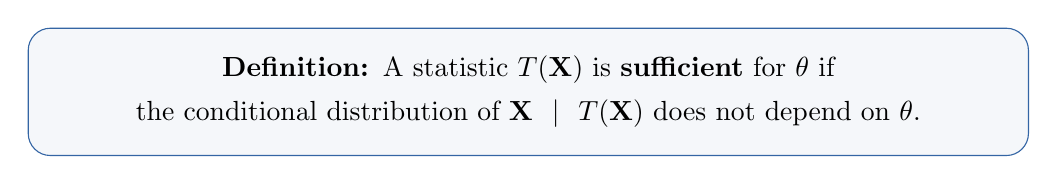
\begin{tikzpicture}
  \node[draw=popblue, fill=popblue!5, rounded corners=8pt, text width=12cm, align=center, inner sep=10pt] {
    \textbf{Definition:} A statistic $T(\mathbf{X})$ is \textbf{sufficient} for $\theta$ if\\[4pt]
    the conditional distribution of $\mathbf{X} \mid T(\mathbf{X})$ does not depend on $\theta$.
  };
\end{tikzpicture}
\end{center}

\vspace{0.2cm}
\begin{center}
\small\textbf{Intuition:} Once you know $T$, the remaining randomness in the data is just noise ---\\
it carries \textbf{no information} about $\theta$. \;$T$ is a ``lossless summary.''
\end{center}
\end{frame}

\begin{frame}
\frametitle{Sufficiency as Data Compression}

\begin{center}
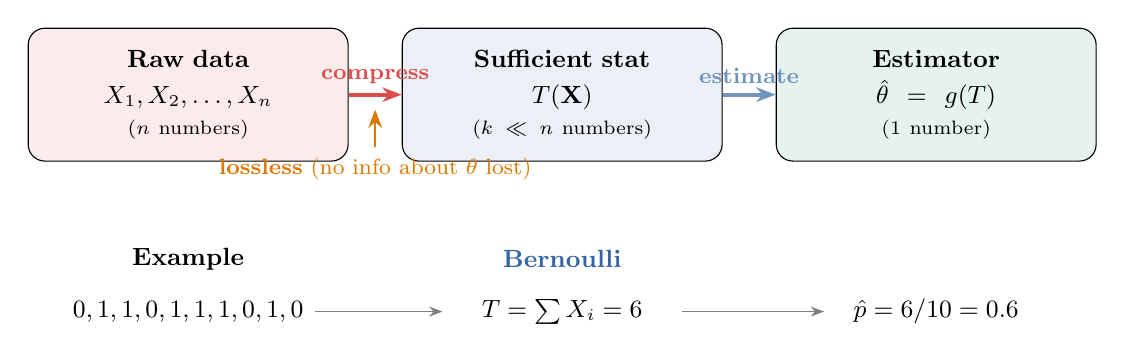
\begin{tikzpicture}[scale=0.95,
  box/.style={draw, rounded corners=6pt, minimum height=1.2cm, align=center, inner sep=8pt, font=\small},
  arrow/.style={-{Stealth[length=7pt]}, line width=1.5pt}
]
  \node[box, fill=sampred!8, text width=3.5cm] (raw) at (-5, 0) {
    \textbf{Raw data}\\[2pt]
    $X_1, X_2, \ldots, X_n$\\
    {\scriptsize ($n$ numbers)}
  };
  \node[box, fill=popblue!10, text width=3.5cm] (suff) at (0, 0) {
    \textbf{Sufficient stat}\\[2pt]
    $T(\mathbf{X})$\\
    {\scriptsize ($k \ll n$ numbers)}
  };
  \node[box, fill=paramgreen!10, text width=3.5cm] (est) at (5, 0) {
    \textbf{Estimator}\\[2pt]
    $\hat\theta = g(T)$\\
    {\scriptsize (1 number)}
  };
  \draw[arrow, sampred!70] (raw) -- (suff) node[midway, above, font=\footnotesize\bfseries] {compress};
  \draw[arrow, popblue!70] (suff) -- (est) node[midway, above, font=\footnotesize\bfseries] {estimate};
  \node[font=\footnotesize, orange1] at (-2.5, -1.0) {\textbf{lossless} (no info about $\theta$ lost)};
  \draw[-{Stealth}, orange1, thick] (-2.5, -0.7) -- (-2.5, -0.2);
  \node[font=\small\bfseries] at (-5, -2.2) {Example};
  \node[font=\small] at (-5, -2.9) {$0,1,1,0,1,1,1,0,1,0$};
  \node[font=\small\bfseries, popblue] at (0, -2.2) {Bernoulli};
  \node[font=\small] at (0, -2.9) {$T = \sum X_i = 6$};
  \node[font=\small] at (5, -2.9) {$\hat{p} = 6/10 = 0.6$};
  \draw[-{Stealth}, gray, thin] (-3.3, -2.9) -- (-1.6, -2.9);
  \draw[-{Stealth}, gray, thin] (1.6, -2.9) -- (3.5, -2.9);
\end{tikzpicture}
\end{center}

\vspace{0.1cm}
\begin{center}
\small The order $(0,1,1,0,1,\ldots)$ doesn't matter for estimating $p$ ---
only the \textbf{total count} matters.
\end{center}
\end{frame}

\begin{frame}
\frametitle{How to Check: Fisher--Neyman Factorization}

\small
\textbf{Theorem:} $T(\mathbf{X})$ is sufficient for $\theta$ if and only if:
$$f(\mathbf{x} \mid \theta) = g\!\left(T(\mathbf{x}),\; \theta\right) \cdot h(\mathbf{x})$$
where $g$ depends on the data \textbf{only through $T$}, and $h$ does not depend on $\theta$.

\vspace{0.15cm}
\textbf{Bernoulli worked example:} $X_1, \ldots, X_n \sim \text{Bern}(p)$, let $T = \sum X_i$.
$$f(\mathbf{x} \mid p) = \prod_{i=1}^n p^{x_i}(1-p)^{1-x_i} = \underbrace{p^{\,\sum x_i}(1-p)^{n - \sum x_i}}_{g(T,\; p)} \cdot \underbrace{1\vphantom{p^{\sum}}}_{h(\mathbf{x})}$$

\vspace{0.1cm}
\begin{center}
\renewcommand{\arraystretch}{1.5}
\begin{tabular}{lll}
  \textbf{Model} & \textbf{Sufficient statistic} & \textbf{Intuition} \\
  \hline
  $\text{Bern}(p)$ & $T = \sum X_i$ & 1 number for 1 parameter \\
  $N(\mu, \sigma^2_0)$ \;($\sigma^2_0$ known) & $T = \bar{X}$ & 1 number for 1 parameter \\
  $N(\mu, \sigma^2)$ \;(both unknown) & $T = (\bar{X},\; S^2)$ & 2 numbers for 2 parameters \\
  \hline
\end{tabular}
\end{center}
\end{frame}

% --- Item 9: Split minimal sufficiency into 2 slides ---
\begin{frame}
\frametitle{Minimal Sufficiency}

\small
The full data $\mathbf{X}$ is always trivially sufficient. But can we compress \textbf{further}?

\vspace{0.15cm}
\begin{center}
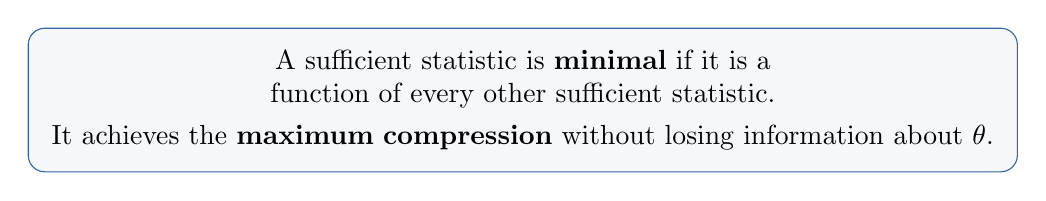
\begin{tikzpicture}
  \node[draw=popblue, fill=popblue!5, rounded corners=6pt, text width=12cm, align=center, inner sep=8pt] {
    A sufficient statistic is \textbf{minimal} if it is a function of every other sufficient statistic.\\[3pt]
    It achieves the \textbf{maximum compression} without losing information about $\theta$.
  };
\end{tikzpicture}
\end{center}

\vspace{0.15cm}
\textbf{Example:} For $X_1, \ldots, X_n \sim N(\mu, \sigma^2_0)$ with $\sigma^2_0$ known:

\vspace{0.1cm}
\begin{center}
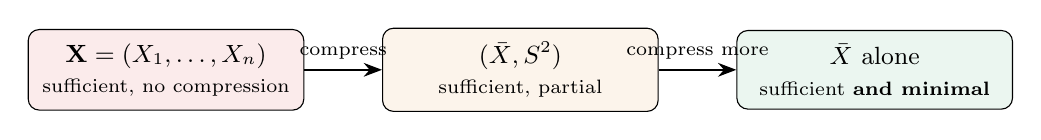
\begin{tikzpicture}[
  sbox/.style={draw, rounded corners=4pt, minimum width=3.5cm, minimum height=0.9cm, align=center, inner sep=5pt, font=\small}
]
  \node[sbox, fill=sampred!8] (full) at (-4.5, 0) {$\mathbf{X} = (X_1, \ldots, X_n)$\\{\scriptsize sufficient, no compression}};
  \node[sbox, fill=orange1!8] (pair) at (0, 0) {$(\bar{X}, S^2)$\\{\scriptsize sufficient, partial}};
  \node[sbox, fill=paramgreen!8] (min) at (4.5, 0) {$\bar{X}$ alone\\{\scriptsize sufficient \textbf{and minimal}}};
  \draw[-{Stealth}, thick] (full) -- (pair) node[midway, above, font=\scriptsize] {compress};
  \draw[-{Stealth}, thick] (pair) -- (min) node[midway, above, font=\scriptsize] {compress more};
\end{tikzpicture}
\end{center}

\vspace{0.15cm}
\begin{center}
\small Since only $\mu$ is unknown, $S^2$ carries no extra information --- $\bar{X}$ alone is enough.
\end{center}
\end{frame}

\begin{frame}
\frametitle{The Rao--Blackwell Theorem}

\small
Why does sufficiency matter for estimation? Because it lets us \textbf{improve} any estimator:

\vspace{0.15cm}
\begin{center}
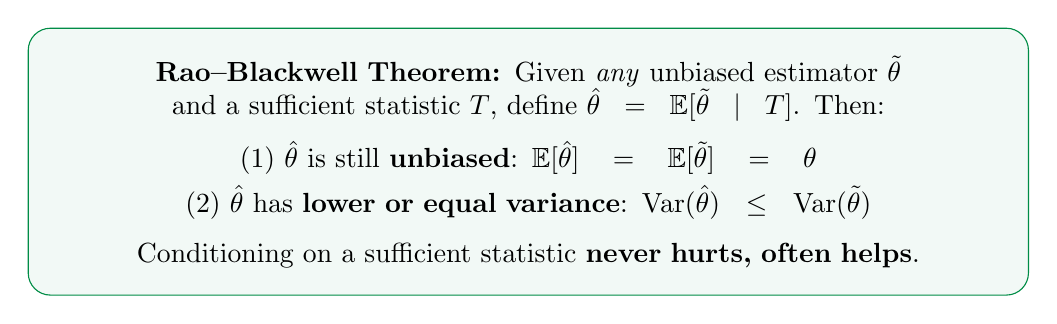
\begin{tikzpicture}
  \node[draw=paramgreen, fill=paramgreen!5, rounded corners=8pt, text width=12cm, align=center, inner sep=10pt] {
    \textbf{Rao--Blackwell Theorem:} Given \textit{any} unbiased estimator $\tilde\theta$\\
    and a sufficient statistic $T$, define $\hat\theta = \mathbb{E}[\tilde\theta \mid T]$. Then:\\[6pt]
    (1) $\hat\theta$ is still \textbf{unbiased}: $\mathbb{E}[\hat\theta] = \mathbb{E}[\tilde\theta] = \theta$\\[3pt]
    (2) $\hat\theta$ has \textbf{lower or equal variance}: $\text{Var}(\hat\theta) \leq \text{Var}(\tilde\theta)$\\[6pt]
    Conditioning on a sufficient statistic \textbf{never hurts, often helps}.
  };
\end{tikzpicture}
\end{center}

\pause
\vspace{0.15cm}
\textbf{Worked example:} $X_1,\ldots,X_n \sim \text{Bern}(p)$, \;sufficient stat $T = \sum X_i$.

\vspace{0.1cm}
\begin{center}
$\underbrace{\tilde{p} = X_1}_{\text{naive: unbiased, Var} = p(1-p)}$
\quad$\xrightarrow{\;\;\mathbb{E}[\,\cdot\mid T\,]\;\;}$\quad
$\underbrace{\hat{p} = \mathbb{E}[X_1 \mid T] = T/n = \bar{X}}_{\text{improved: unbiased, Var} = p(1-p)/n}$
\quad\textcolor{paramgreen}{$\boldsymbol{\times n}$ \textbf{better!}}
\end{center}
\end{frame}

\begin{frame}
\frametitle{What Does $\mathbb{E}[\tilde\theta \mid T]$ Actually Mean?}

\small
\textbf{Concrete example:} $X_1, X_2, X_3 \sim \text{Bern}(p)$, \;$T = X_1 + X_2 + X_3$, \;$\tilde{p} = X_1$.

\vspace{0.15cm}
Suppose someone tells you $T = 2$ (two successes). Which data vectors give $T = 2$?

\vspace{0.1cm}
\begin{center}
\renewcommand{\arraystretch}{1.4}
\begin{tabular}{cccc}
  $(X_1, X_2, X_3)$ & $T$ & $\tilde{p} = X_1$ & Equally likely? \\
  \hline
  $(1, 1, 0)$ & $2$ & $1$ & Yes \\
  $(1, 0, 1)$ & $2$ & $1$ & Yes \\
  $(0, 1, 1)$ & $2$ & $0$ & Yes \\
  \hline
\end{tabular}
\end{center}

\pause
\vspace{0.05cm}
$$\mathbb{E}[X_1 \mid T = 2] = \frac{1 + 1 + 0}{3} = \frac{2}{3} = \frac{T}{n} \quad\textcolor{paramgreen}{\checkmark}$$

\vspace{0.05cm}
\begin{center}
\fcolorbox{popblue}{popblue!5}{\parbox{11cm}{\centering\small
  \textbf{``Condition on $T$''} means: average $\tilde\theta$ over all data configurations\\
  that produce the same value of $T$. The noise (which specific $X_i$'s\\
  are 1 vs 0) gets averaged away. Only the useful part ($T$) survives.
}}
\end{center}
\end{frame}

\begin{frame}
\frametitle{Why Does Rao--Blackwell Work?}

\small
The key is the \textbf{law of total variance} (a.k.a.\ Eve's law):
\vspace{-0.2cm}
$$\text{Var}(\tilde\theta) = \underbrace{\mathbb{E}\!\left[\text{Var}(\tilde\theta \mid T)\right]}_{\text{``useless'' noise}\;\geq\, 0} + \text{Var}\!\left(\underbrace{\mathbb{E}[\tilde\theta \mid T]}_{\hat\theta}\right)$$

\pause
\vspace{-0.2cm}
Since the first term $\geq 0$, we immediately get:
$\;\boxed{\text{Var}(\tilde\theta) \;\geq\; \text{Var}(\hat\theta)}$

\vspace{0.05cm}
\begin{center}
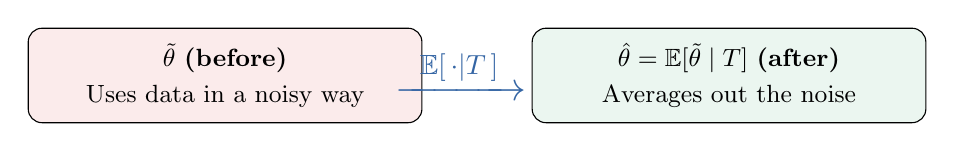
\begin{tikzpicture}[
  box/.style={draw, rounded corners=5pt, minimum width=5cm, minimum height=1.2cm, align=center, inner sep=5pt, font=\small}
]
  \node[box, fill=sampred!8] at (-4.2, 0) {
    $\tilde\theta$ \textbf{(before)}\\[2pt]
    Uses data in a noisy way
  };
  \node[font=\Large\bfseries, popblue] at (-1.2, 0) {$\xrightarrow{\;\;\mathbb{E}[\,\cdot\mid T\,]\;\;}$};
  \node[box, fill=paramgreen!8] at (2.2, 0) {
    $\hat\theta = \mathbb{E}[\tilde\theta \mid T]$ \textbf{(after)}\\[2pt]
    Averages out the noise
  };
\end{tikzpicture}
\end{center}

\vspace{-0.05cm}
\begin{center}
\fcolorbox{popblue}{popblue!5}{\parbox{11cm}{\centering\small
  \textbf{Intuition:} $T$ captures all the useful information about $\theta$.
  Conditioning on $T$ removes the ``useless'' randomness (the part that
  doesn't tell us about $\theta$). What's left is a cleaner estimator.
}}
\end{center}
\end{frame}

\begin{frame}
\frametitle{Finding Minimal Sufficient Statistics}

\small
\textbf{Theorem (Likelihood Ratio Criterion):} $T(\mathbf{X})$ is minimal sufficient iff for all $\mathbf{x}, \mathbf{y}$:

$$T(\mathbf{x}) = T(\mathbf{y}) \quad\Longleftrightarrow\quad \frac{f(\mathbf{x} \mid \theta)}{f(\mathbf{y} \mid \theta)} \;\text{does not depend on}\; \theta$$

\vspace{0.15cm}
\textbf{Bernoulli example:} $X_1, \ldots, X_n \sim \text{Bern}(p)$.

$$\frac{f(\mathbf{x} \mid p)}{f(\mathbf{y} \mid p)}
= \frac{p^{\sum x_i}(1-p)^{n-\sum x_i}}{p^{\sum y_i}(1-p)^{n-\sum y_i}}
= \left(\frac{p}{1-p}\right)^{\!\sum x_i - \sum y_i}$$

Free of $p$ $\;\Longleftrightarrow\;$ $\sum x_i = \sum y_i$.
\;\;So $T = \sum X_i$ is \textbf{minimal sufficient} for $p$. \;\textcolor{paramgreen}{$\checkmark$}

\vspace{0.2cm}
\begin{center}
\fcolorbox{orange1}{orange1!5}{\parbox{11cm}{\centering\small
  \textbf{Recipe:} Write the likelihood ratio $f(\mathbf{x}\mid\theta)/f(\mathbf{y}\mid\theta)$.\\
  Find which function of the data must match for the ratio to lose its $\theta$-dependence.\\
  That function is the minimal sufficient statistic.
}}
\end{center}
\end{frame}

% ============================================================
\section{Exponential Family}

\begin{frame}
\frametitle{The Exponential Family: A Unifying Framework}

\small
All our examples --- Bernoulli, Normal, Poisson, Exponential --- share one structure:

$$\boxed{f(x \mid \theta) = h(x)\;\exp\!\Big(\eta(\theta)\,T(x) - A(\theta)\Big)}$$

\vspace{-0.1cm}
\begin{center}
\renewcommand{\arraystretch}{1.5}
\begin{tabular}{lccc}
  \textbf{Distribution} & \textbf{Natural param}~$\eta(\theta)$ & $T(x)$ & \textbf{Suff.\ stat} ($n$ obs) \\
  \hline
  $\text{Bern}(p)$ & $\log\frac{p}{1-p}$ & $x$ & $\sum X_i$ \\[1pt]
  $N(\mu,\sigma_0^2)$ \;($\sigma_0^2$ known) & $\mu/\sigma_0^2$ & $x$ & $\sum X_i$ \\[1pt]
  $\text{Pois}(\lambda)$ & $\log\lambda$ & $x$ & $\sum X_i$ \\[1pt]
  $\text{Exp}(\lambda)$ & $-\lambda$ & $x$ & $\sum X_i$ \\
  \hline
\end{tabular}
\end{center}

\vspace{0.1cm}
\begin{center}
\fcolorbox{popblue}{popblue!5}{\parbox{11cm}{\centering\small
  \textbf{Pattern:} For single-parameter families, $T(x) = x$. The sufficient statistic\\
  for $n$ observations is always $\sum T(X_i)$ --- straight from the factorization theorem!
}}
\end{center}
\end{frame}

% --- Item 10: Fix exponential families slide ---
\begin{frame}
\frametitle{Why Exponential Families Are Special}

\small
Nearly every nice property we've discussed is \textbf{automatic} in exponential families:

\vspace{0.05cm}
\begin{center}
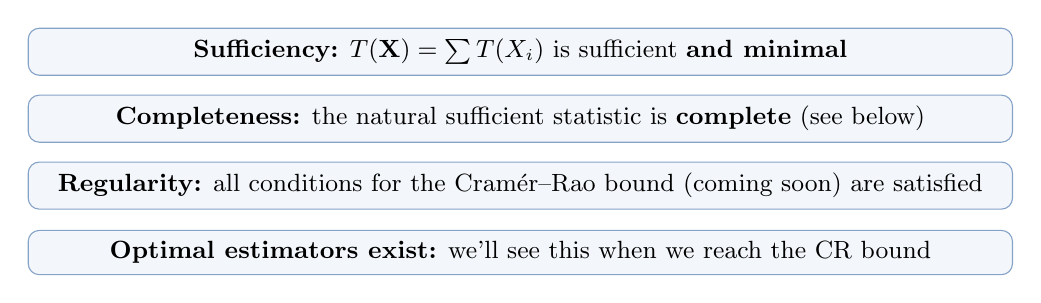
\begin{tikzpicture}[
  pbox/.style={draw=popblue!60, fill=popblue!6, rounded corners=4pt, minimum width=12.5cm, align=left, inner sep=4pt, font=\small}
]
  \node[pbox] at (0, 1.2) {\textbf{Sufficiency:} $T(\mathbf{X}) = \sum T(X_i)$ is sufficient \textbf{and minimal}};
  \node[pbox] at (0, 0.35) {\textbf{Completeness:} the natural sufficient statistic is \textbf{complete} (see below)};
  \node[pbox] at (0, -0.5) {\textbf{Regularity:} all conditions for the Cram\'er--Rao bound (coming soon) are satisfied};
  \node[pbox] at (0, -1.35) {\textbf{Optimal estimators exist:} we'll see this when we reach the CR bound};
\end{tikzpicture}
\end{center}

\vspace{0.05cm}
\begin{center}
\fcolorbox{paramgreen}{paramgreen!5}{\parbox{12cm}{\centering\small
  \textbf{Completeness} means: if $\mathbb{E}_\theta[g(T)] = 0$ for all $\theta$, then $g(T) = 0$ a.s.
  $\to$ \textbf{no non-trivial unbiased estimator of zero} based on $T$.\\[3pt]
  \textbf{Lehmann--Scheff\'e:} An unbiased estimator based on a \textbf{complete} sufficient
  statistic is the \textbf{unique best} unbiased estimator (UMVUE).
  For exp.\ families, $\sum T(X_i)$ is always complete $\Rightarrow$ UMVUE exists!
}}
\end{center}
\end{frame}


% ============================================================
\section{Summary}

\begin{frame}
\frametitle{Homework}
\begin{enumerate}
  \item Show that $\bar{X}$ is unbiased for $\mu$ and compute its MSE.

  \vspace{0.2cm}
  \item Show that $\hat\sigma^2_n = \frac{1}{n}\sum(X_i - \bar{X})^2$ is biased for $\sigma^2$. Find the bias.

  \vspace{0.2cm}
  \item Suppose you shrink $\bar{X}$ toward 0: $\;\hat\mu_c = c\bar{X}$ for $0 < c < 1$.\\
    Find the bias, variance, and MSE as functions of $c$.\\
    For what value of $c$ is MSE minimized? Is the optimal estimator biased?

  \vspace{0.2cm}
  \item Use the factorization theorem to show that $T = \sum X_i$ is a sufficient statistic\\
    for $\lambda$ when $X_1, \ldots, X_n \sim \text{Poisson}(\lambda)$.
\end{enumerate}
\end{frame}

\begin{frame}
\begin{center}
  {\Huge\bfseries\textcolor{popblue}{Questions?}}
\end{center}
\end{frame}

\end{document}
